%!TEX root = main.tex
\chapter{Introduction}
This thesis will present a design-science project where the goal was to design a web tool for use as support for learning and reflection in agile project development teams. The purpose of the tool is to make collecting of experiences easier during a project development process, and enhance learning outcomes from the reflection sessions. The tool will collect data from the development process and present them to the users in a tailored way. Users can annotate these data with their own experiences, including connecting feelings to these experiences. The web tool will present these data and experiences for use in both individual and collaborative reflection settings. The challenge will be to collect, annotate and present the data in a way that helps the learner to understand what they have experienced and learn from these experiences. That is helping them reflect on the experiences made and learn from them. Boud et.al\cite{boudreflection1985} presents that; \emph{reflection is a process where the experience is revisited, feelings are re-attended and the experience is re-evaluated}. This means that it is important to tailor reflection in order to support and achieve learning.

\section{Context and background}
For many years now, agile methods in software development have been widely used in software development teams. The agile manifesto presents a principle which states that an agile team should regularly reflect on how to become more effective, and tune its behavior accordingly\cite{Beck2001}. Continuously improving through introspection is a vital part of agile methods and is applied in f.ex retrospectives\cite{Beck1999, Derby2006, Maham2008}. Cockburn impose that a vital part of agile practice should be conducting regular retrospective workshops aimed at reflection and process tune-up\cite{Cockburn2006}. Agile methods focus on continuous iterations repeating the same development steps, and thus progressing. Retrospectives in agile development processes are most often performed after each iteration. This is done by gathering the team and reflecting on their way of working, so that improvements for the next iteration can be identified.\cite{Derby2006, Drury2011}. This enables agile self-governing teams to react quickly to changes, and make modifications accordingly\cite{Drury2011}. Retrospectives could also support communication and interaction within the team, which is important for agile development. There are however shortcomings of applying retrospectives in agile teams. Agile teams tend to focus primarily on short-term issues that were identified for a single iteration, and not on long-term strategic issues\cite{Drury2011}. 
In this thesis we will develop a tool in order to address the challenges described above. The tool is aimed at supporting reflection by a scaffolded collection of relevant project artifacts, and prompting users to annotate these artifacts with their experiences and feelings. The tool is designed and developed for software development projects using an agile method, and will be evaluated with an agile team taking a software development course at NTNU. 

\subsection{Domain}
• Motivation: Brief description of the research domain and the problem that one
wants to address. It should tell the reader why working on this project is worth
doing.

\subsection{Core Concepts}
Explain

\subsubsection{Reflection}
The goal is to offer technology that not only makes information search and collection efficient, but also support reflection in a collaborative session. Through reflection learning can be achieved and users can collaborate on gathering information for experiences and the ability to reflect over experiences by displaying data in different methods this might enhance the reflection ability and letting the user view data in another way.

\subsubsection{Learning from experience}

\subsubsection{Software development}
% Trekke inn modellen til birgit? YES!
Software developers generate a lot of data when developing software, when commit data to versioncontrol systems or closing tasks or issues in a project management tool. During a development cycle, tasks is distributed among the developers and they make decisions either individualy or in plural. Normal this set of data is never looked at again, but they contain vital information on choices the developers make at some point in there development. It is important to make collecting of information a part of developers normal day-to-day activities based on the model\cite{Krogstie2009}.

\subsubsection{Version controll systems}
Explain it.

%!TEX root = main.tex
\section{Research Question}

%%%%%%%%%%%%%%%%%%%%%%
% HER ER DET MYE RART?
% Oppdatere?
% The thesis should introduce versiontracking control here, and introduce Github as an example of such a tool. Need to explain why we chose Github(api etc.)
%%%%%%%%%%%%%%%%%%%%%%
\begin{itemize}
	\item How to promote experienced-based learning from reflection based on project artifatcs collected from version-control systems?
	\begin{itemize}
		\item How to scaffold collection of data inorder to promote daily reflection?
		% Dette virker litt langt/det går kanskje inn under et av de andre spm?\item How to give individuals an outline of what they have contributed with as individuals compared to others in a project with multiple contributors for individual reflection?
		\item How to collect daily experiences for use in collaborativ reflection sessions?
		\item How to increase the tendency to reflect on experiences, both individually and as a team? 
		\item How to bring together contributions from multiple users, possibly using different conceptualization of the work process? 
		\item How to support cooperation around these representations?
	\end{itemize}
\end{itemize}
%!TEX root = main.tex
%
% ### Research Method
% Where are we getting requirements from?  
% What will guide our design?  
% How will we evaluate the tool?  
%
\section{Research Method}

% Lage et diagram som http://daim.idi.ntnu.no/masteroppgave?id=6231 og Timeline masteroppgaven gjør. Altså hvordan vi har gått frem underveis. Skriv så litt om hver periode, hva vi har gjort etc. Veldig likt timeline bare ikke så mye. Dropp såå alle de subsectionsa under. Går sikkert an å bake inn litt fra de ulike stedene, de bør jo nevnes. F.eks research rigor etc. 

The \emph{Design-Science Research Guidelines} presented in \cite{Esearch2004} the  will serve as the basis of this design-science research. The guidelines were created in order to assist researchers to understand the necessary requirements for effective design-science research. We will also be using the regulative cycle\cite{wieringa}.
\begin{figure}[!htpb]
\label{regulativecycle}
\centering
	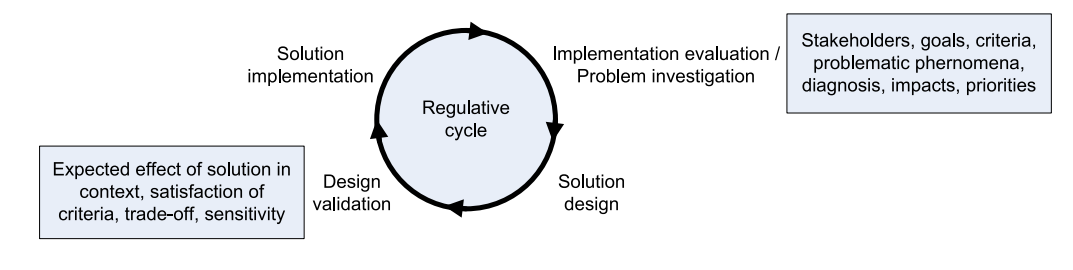
\includegraphics[width=\textwidth]{regulativecycle}
\caption{Regulativecycle development in Design-Science research}
\end{figure}

\subsection{Development steps}
Our researchmodel shows our thesis from initial idea to evaluation and results:

\begin{figure}[!htpb]
\label{researchmodel}
\centering
	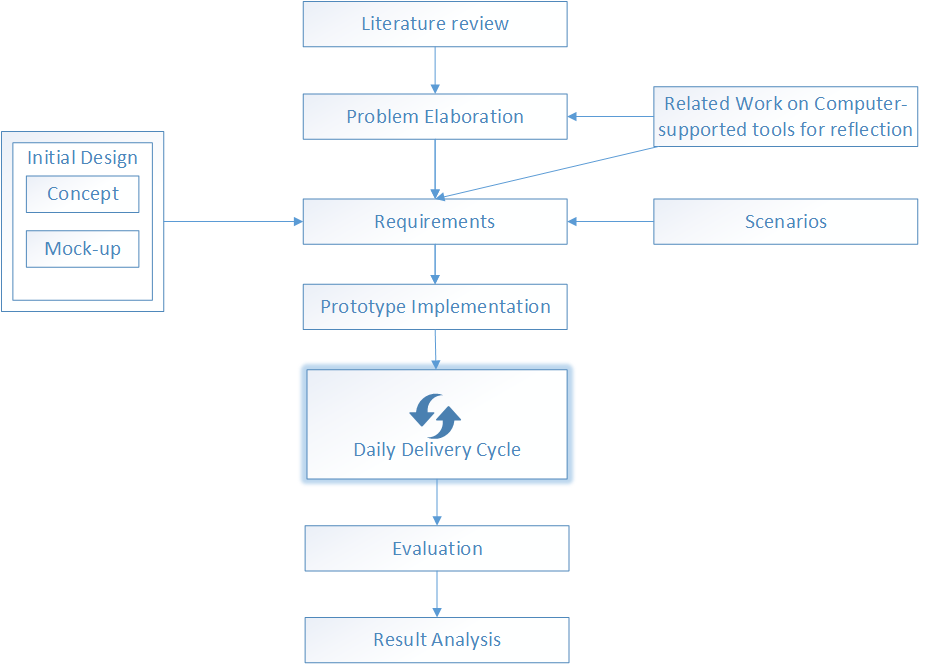
\includegraphics[width=\textwidth]{researchmodel_and_iterationcycle}
\caption{The researchmodel}
\end{figure}

\begin{figure}[!htpb]
\label{iterationprocess}
\centering
	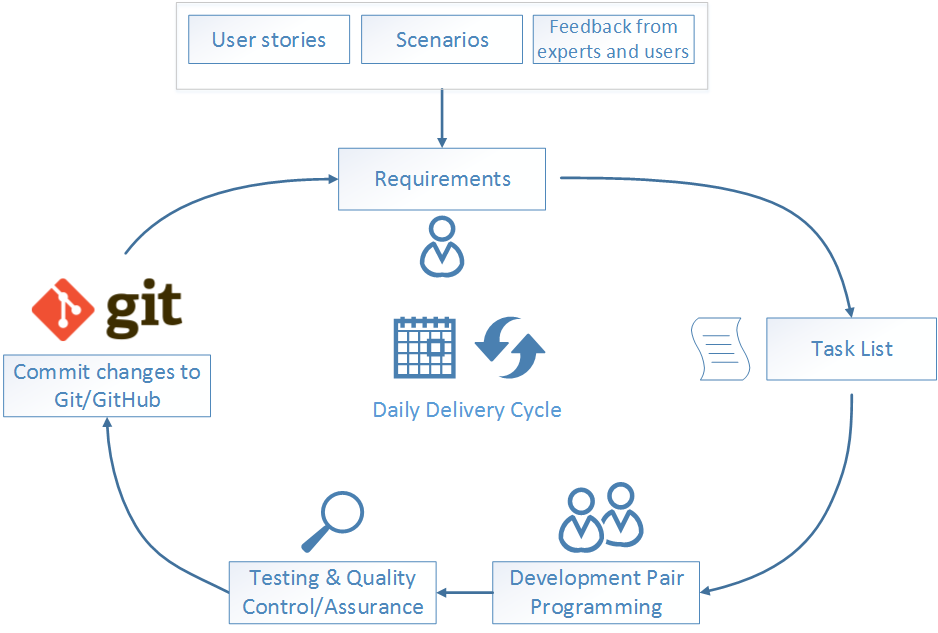
\includegraphics[width=\textwidth]{iterationprocess}
\caption{The daily delivery cycle}
\end{figure}

%Evaluation:
%Core questions described in the toolbox, 9.1:
%Demographic questions, usage of the app, most relevant app-specific questions - choosing the questions that are most important to our thesis. 
%In addition we will use the reflection scale, shown in 9.1.4 both before and after the evaluation period, in order to measure the effect on the tendency to reflect on past
%experiences. Finally we will include the learning outcomes questions and the work behaviour questions, after the evaluation period. 


%Evaluation with the students in IT2901: 
%Students will use the tool for two weeks, daily individual use and as a team after the two week period. 
%For scenario 2 we will require a team of at least 3 people in order to test. 
%The first scenario does not require anything but a github repository. 

\subsection{Design as an artifact}
By definition, the result of design-science research in Information Science is:
\begin{quote}
A purposeful IT artifact created to address an important organizational problem. It must be described effectively, enabling its implementation and application in an appropriate domain.
\end{quote}
\cite{Markus et al. 2002} identified that a developed artifact is only significant if there is questions like: Can it be constructed, can it perform appropriately and is the result important to the information science community. 
We will create a proof of concept prototype tool for promoting experienced-based learning from reflection based on project artifacts collected from version-control systems. Our goal was to create a tool that can discover new capabilites in the domain of reflection and experience-based learning, as well as support the existing capabilities in an efficient way. Evaluating the tool in \emph{real use} situations is necessary in order to discover if the artifact can enhance the reflection process as it is today. 

\subsection{Problem relevance}
We want to explore how the collection and scaffolding of experiences connected to project artifacts can support collaborative reflection sessions. In order to revisit and learn from previous experiences we want to collect and scaffold experiences from users daily. Experiences and memories change over time, so collecting these experiences as quickly as possible is important. The tool will keep a copy of these experiences in order for users to revisit them at a later date, be it individually or in collaborative reflection sessions. These notes will be collected based on tags that are related to the experience being reviewed \cite{Hassan-montero2006}

\subsection{Evaluation}
Table 2 in \cite{Esearch2004} will be used as guidelines for evaluation of our prototype. 
During evaluation we will be using parts of the evaluation toolbox published by MIRROR\footnote{\url{http://www.mirror-project.eu/showroom-a-publications/downloads/finish/5/67}}. This toolbox is a specification of evaluation methodology and research tooling. 

\subsubsection{Observational}
Before and after the user evaluation of the tool, all test-subjects will be given a form with a set of questions to evaluate the application. We will be using core demographic questions, app usage, the most relevant app-specific questions, and also the reflection scale [\ref{reflectionscale}] from the toolbox. The reflection scale assesses participants' general tendency to reflect and the importance they place on reflection. Using this scale, allows us to see whether using the tool prime people to reflect more. Meaning: Does the tool increase the users tendency to reflect on experiences, both individually and as a team. Measuring this before and after using the tool implementation, allows us to measure the expected increase. \\*
Finally we will include the learning outcomes questions and the work behaviour questions, after the evaluation period.  

\subsubsection{Analytical}
We will perform a dynamic analysis on the data collected from server and user feedback. During use the application will provide simple usage-patterns on how the users use the application.
This will also help us in the analysis of the applications performance as well as its usefulness in the reflection and learning domains

\subsubsection{Testing}
During development we will continuously test the tool  to ensure that the user experience is as expected, as a means of quality assurance.
White Box testing will be executed during development of the application with artificial data to ensure that the function is working properly and as specified. 

\subsubsection{Descriptive}
Evaluation proposal with the students in IT2901 - A project course taken by computer science students on the Norwegian University of Science and Technology (NTNU). 
Students that accept to evaluate our tool, will use it for two weeks, with daily individual use and as a team after the two week period. This will allow us to measure the usage of our scenarios. 

Requirements: 
The first scenario does not require anything but a github repository and is doable both for single and for multiples in teams.
For scenario 2 we will require a team of at least 3 people in order to collect enough data. 
We have continuously been using and evaluating the tool ourselves, also a fellow student has been using it for a couple of weeks, so we have some additional evaluation
data also.

\subsection{Research Contributions}
The main goal is to create a proof of concept application that will help users reflect on their past experiences individually and in collaborative reflection sessions by collecting experiences daily and revisiting them at any time. We will analyse the users experience and the evaluation results  in order to draw a conclusion on if multiple representations might help the users to reflect on their past experiences in a collaborative session.

\subsection{Research Rigor}
We will test the tool with a group of experts in the fields relevant and gather data during testing with this group and use this to evaluate the usefulness of the tool. This will serve as a good basis for analysis, triangulate and evaluate to look for relevant research results elsewhere.

\subsection{Design as a redsearch process}
The application will be developed in two main parts, which is central to this research. The first part is development and the second is testing/evaluating the results.

Implementing the application will be developed in development cycles; The first goal will be to develop ideas and a basic mock-up of the application and its design. The second goal will be to implement basic features. Implementation of the individual and collaboration features will then be developed on the basis of feedback from the first cycles. Finally we will focus on integrating all the features into the final system, and create a tool for individual and collaborative reflection use. We will use the tool ourselves during development, as it would be used in a real world environment. In this way we will ensure that all functionality is working as expected, and also identify limitations in the design. 

Finally we will perform the case study evaluation with computer-science students, and the expert review. Evaluating these separately will provide two sets of feedback which we can compare in order to possibly see if any patterns emerge. 

\subsection{Research communication}
The proof of concept application will be available for testing along with a user guide, the whole process will be well documented and our research results will be made available.
Any limitations identified  will be documented along with the research results. 




\section{Results}
\section{Outline}